\appendix

\chapter{Anhang A - Wahl der optimalen Hyperparameter}
Dieser Anhang beinhaltet die Dokumentation der Auswahl der optimalen Hyperparameter, die nicht zum gewünschten Erfolg geführt hat.


\subsection*{Lernrate}
Zunächst wurde die Lernrate angepasst. Neben der bereits definierten Lernrate von $4 * 10^{-4}$, beziehungsweise $4e-4$ in der Terminologie der ML-Agents-Konfigurationsdatei, wurden eine geringere Lernrate von $5e-5$ und eine höhere Lernrate von $8e-3$ verwendet. Die Ergebnisse sind in den folgenden Abbildungen zu erkennen.

\begin{figure}[H]
\centering
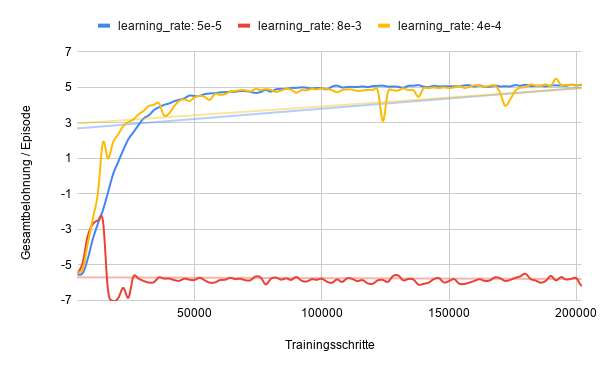
\includegraphics[scale=0.6]{images/training/base_results/result_learningrate_rewards.png}
\caption{Belohnungsverlauf, Anpassung von \Fachbegriff{learning\_rate}}
\label{fig:result_learningrate_rewards}
\end{figure}

\begin{figure}[H]
\centering
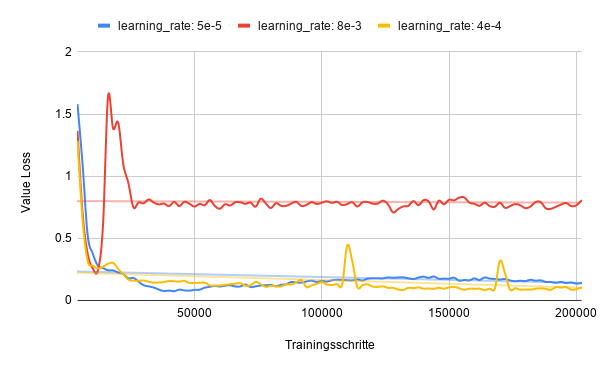
\includegraphics[scale=0.6]{images/training/base_results/result_learningrate_loss.png}
\caption{Verlauf des Value Loss, Anpassung von \Fachbegriff{learning\_rate}}
\label{fig:result_learningrate_loss}
\end{figure}

\begin{figure}[H]
\centering
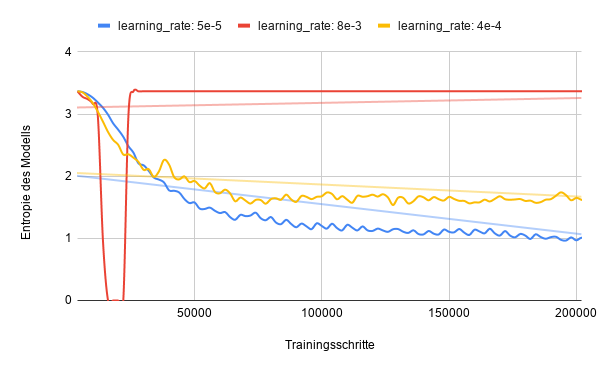
\includegraphics[scale=0.6]{images/training/base_results/result_learningrate_entropy.png}
\caption{Entropieverlauf, Anpassung von \Fachbegriff{learning\_rate}}
\label{fig:result_learningrate_entropy}
\end{figure}

Man erkennt deutlich, dass mit $8e-3$ eine deutlich zu hohe Lernrate gewählt wurde. Zwar steigt die Belohnungsfunktion anfangs im Vergleich leicht schneller, doch schließlich fällt die Kurve rapide ab und bleibt anschließend auf einem sehr schlechten Niveau. Es ist zu vermuten, dass durch den hohen Wert beim Gradientenaufstieg Maxima übersprungen werden. Die Policy wird also jeweils zu stark geändert. Das führt zu einem völlig unbrauchbaren Ergebnis. Auch anhand der Entropie und dem Value Loss wird dies deutlich.
Die Lernrate des Basistrainings mit dem Wert $4e-4$ führt zu einem deutlich besseren Ergebnis. Im Vergleich zu der Kurve mit einer Lernrate von $5e-5$ steigt sie schneller, weist jedoch zwischenzeitlich deutliche Einbrüche auf. Insgesamt wurde jedoch ein ähnlich gutes Ergebnis erzielt, da die Belohnungen nach etwa 100.000 Schritten fast identische Werte annehmen. Der Value Loss erreicht für die niedrigere Lernrate leicht schlechtere Ergebnisse, jedoch ist für die niedrige Lernrate auch zum Ende des Graphen hin eine Abnahme zu erkennen, während der Graph der mittelhohen Lernrate ein Plateau erreicht. Daher wird davon ausgegangen, dass sich der Value Loss mit einer höheren Anzahl von Trainingsschritten weiter verbessert.
Die Entropie zeigt deutlich, dass mit der geringeren Lernrate weniger zufällige Entscheidungen getroffen werden. Aufgrund dieser Tatsache und der deutlich höheren Stabilität der Belohnungsfunktion wird die Lernrate für das finale Training auf den Wert $5e-5$ festgelegt. Generell ist anzunehmen, dass mit einer geringeren Lernrate stets mindestens äquivalente Ergebnisse erzeugt werden können, sich aber insgesamt ein stabileres Training ergibt. Die Anzahl der Trainingsschritte kann dabei problemlos erhöht werden. Die höhere Steigung der Belohnungsfunktion für die mittelhohe Lernrate ist nicht relevant - das Endergebnis und die Stabilität des Trainings spielen eine höhere Rolle.


\subsection*{Anzahl der Schichten}
Weiterhin wurde die Anzahl der Schichten im neuronalen Netz angepasst. Das Basistraining beinhaltet ein Netz mit drei Schichten. Zusätzlich wurden zwei, vier und fünf Schichten getestet.

\begin{figure}[H]
\centering
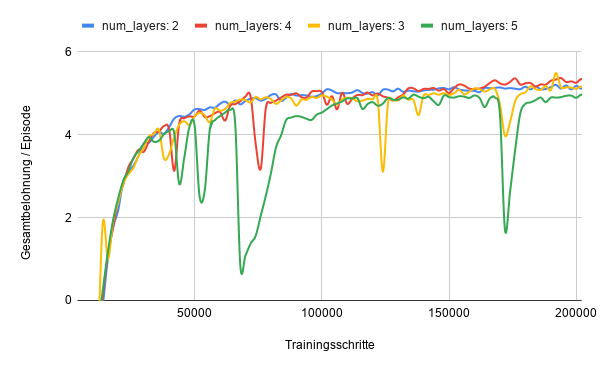
\includegraphics[scale=0.6]{images/training/base_results/result_layers_reward.png}
\caption{Belohnungsverlauf, Anpassung von \Fachbegriff{num\_layers}}
\label{fig:result_layers_reward}
\end{figure}

\begin{figure}[H]
\centering
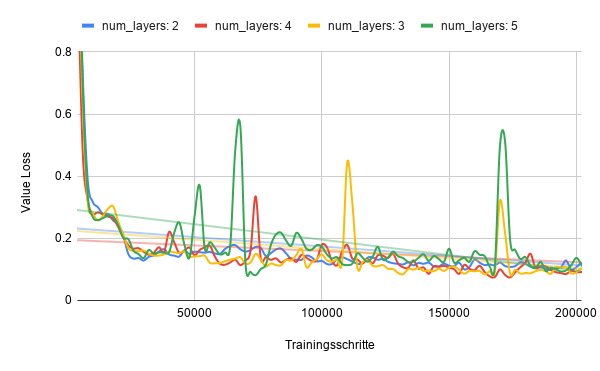
\includegraphics[scale=0.6]{images/training/base_results/result_layers_loss.png}
\caption{Verlauf des Value Loss, Anpassung von \Fachbegriff{num\_layers}}
\label{fig:result_layers_loss}
\end{figure}

\begin{figure}[H]
\centering
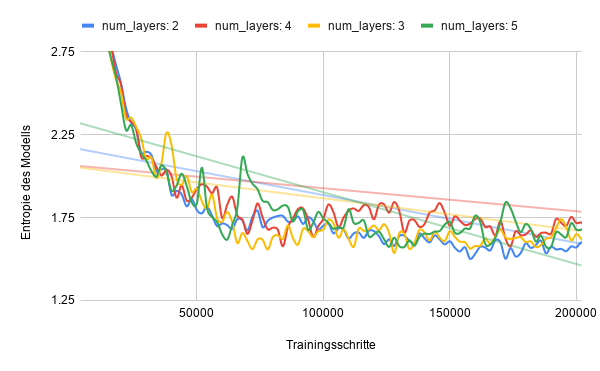
\includegraphics[scale=0.6]{images/training/base_results/result_layers_entropy.png}
\caption{Entropieverlauf, Anpassung von \Fachbegriff{num\_layers}}
\label{fig:result_layers_entropy}
\end{figure}

Anhand der Belohnungsfunktion kann man erkennen, dass die Verwendung von vier Schichten zu dem höchsten Reward führt. Insgesamt ist der allgemeine Verlauf der Funktionen ähnlich. Wenn allerdings fünf Schichten verwendet werden, entstehen starke Schwankungen und Einbrüche sowie eine insgesamt niedrigere Belohnung. Das lässt sich auch anhand des Entropieverlaufs und dem Value Loss erkennen. Die Nutzung von fünf Schichten ist daher nicht akzeptabel. Vier verwendete Schichten führen zu einem leicht erhöhten Entropieverlauf und einer Value Loss-Funktion, die sich mit den anderen Verläufen deckt. Da insgesamt aber eine höhere Belohnung erzielt wird, werden für das finale Training vier Schichten verwendet.   


\subsection*{Anzahl der Neuronen}
Die Anzahl der Neuronen wurde auf eine Anzahl von 128, 256, 384 und 512 festgelegt. Aufgrund der Erkenntnis des letzten Abschnitts wurden hierfür vier Schichten genutzt.

\begin{figure}[H]
\centering
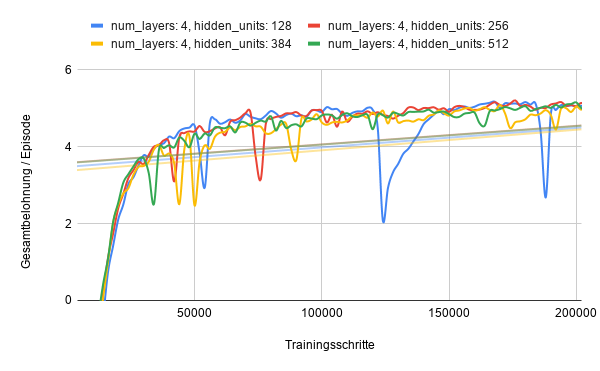
\includegraphics[scale=0.6]{images/training/base_results/result_neurons_rewards.png}
\caption{Belohnungsverlauf, Anpassung von \Fachbegriff{hidden\_units}}
\label{fig:result_neurons_rewards}
\end{figure}

\begin{figure}[H]
\centering
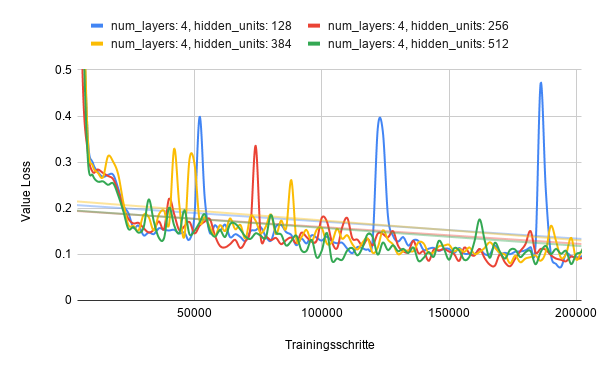
\includegraphics[scale=0.6]{images/training/base_results/result_neurons_loss.png}
\caption{Verlauf des Value Loss, Anpassung von \Fachbegriff{hidden\_units}}
\label{fig:result_neurons_loss}
\end{figure}

\begin{figure}[H]
\centering
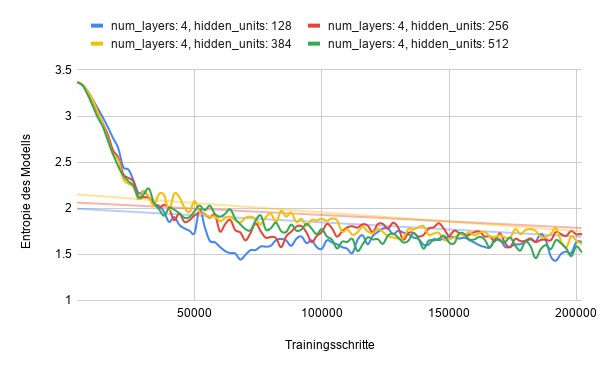
\includegraphics[scale=0.6]{images/training/base_results/result_neurons_entropy.png}
\caption{Entropieverlauf, Anpassung von \Fachbegriff{hidden\_units}}
\label{fig:result_neurons_entropy}
\end{figure}

An dem Verlauf der akkumulierten Belohnungen kann man erkennen, dass insgesamt sehr ähnliche Ergebnisse für die jeweils höchste Belohnung erzielt werden. Die Nutzung von 128 Neuronen pro Schicht führt allerdings zu häufigeren Einbrüchen, da durch die geringere Anzahl der Neuronen weniger kleinschrittige Änderungen des Modells möglich sind. 128 Neuronen sind daher nicht ausreichend. Für 384 und 512 Neuronen wird ein insgesamt leicht schlechteres und instabileres Ergebnis erreicht, als bei 256. Mit 384 Neuronen wurde also eine zu hohe Anzahl gewählt.

Die genannten Einbrüche mit 128 Neuronen sind ebenfalls in der Value Loss-Funktion zu betrachten. Die beiden Kurve für 256 und 384 Neuronen erreichen hingegen sehr ähnliche Ergebnisse. Ebenso ähneln sich deren Funktionen für die Entropie des Modells. Hier ist weiterhin zu erkennen, dass durch die Nutzung von weniger Neuronen eine schnellere Konvergenz erreicht wird, nach etwa 150.000 Trainingsschritten erreichen die Kurven jedoch ein ähnliches Level.
Es besteht zusätzlich die Vermutung, dass bei einer Erhöhung der Anzahl der Neuronen mehr Trainingsschritte benötigt werden, um das Modell hinreichend anzupassen. Daher wird ein erweiterter Trainingslauf in der folgenden Abbildung \ref{fig:result_neurons_rewards_extended} betrachtet:

\begin{figure}[H]
\centering
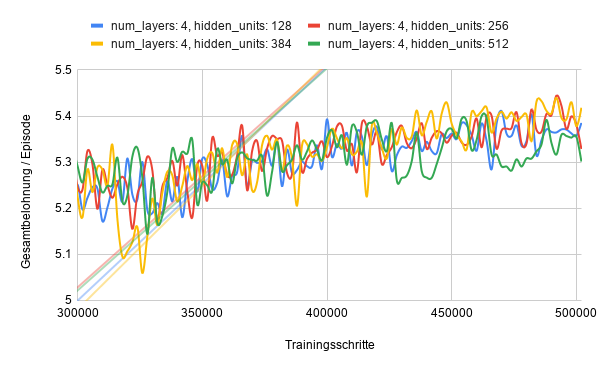
\includegraphics[scale=0.7]{images/training/base_results/result_neurons_rewards_extended.png}
\caption{Erweiterter Belohnungsverlauf, Anpassung von \Fachbegriff{hidden\_units}}
\label{fig:result_neurons_rewards_extended}
\end{figure}

In der Grafik ist zu erkennen, dass sich das Ergebnis für höhere Mengen von Neuronen mit steigender Anzahl von Trainingsschritten leicht verbessert. Aufgrund dieses Verlaufs und dem schlechteren Verlauf des Trainings mit 384 Neuronen werden insgesamt 256 Neuronen pro Schicht für das finale Training genutzt.


\subsection*{Rekurrentes Netz}
Der Parameter \Fachbegriff{use\_recurrent} wird auf \Fachbegriff{true} gesetzt, um ein rekurrentes neuronales Netz zu nutzen. Dabei wird eine \Fachbegriff{memory\_size} von der Größe $128$ genutzt. Die Ergebnisse sind in den folgenden Abbildungen zu sehen.

\begin{figure}[H]
\centering
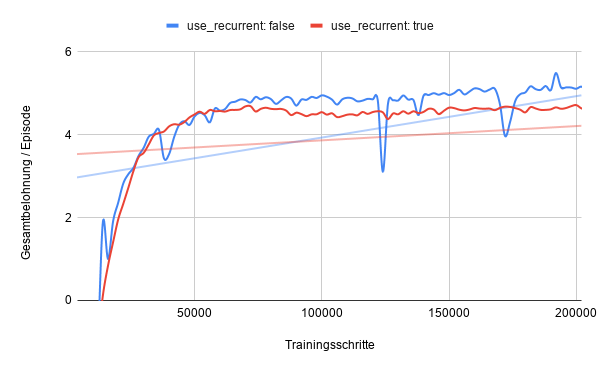
\includegraphics[scale=0.6]{images/training/base_results/result_userecurrent_rewards.png}
\caption{Belohnungsverlauf, Anpassung von \Fachbegriff{use\_recurrent}}
\label{fig:result_userecurrent_rewards}
\end{figure}

\begin{figure}[H]
\centering
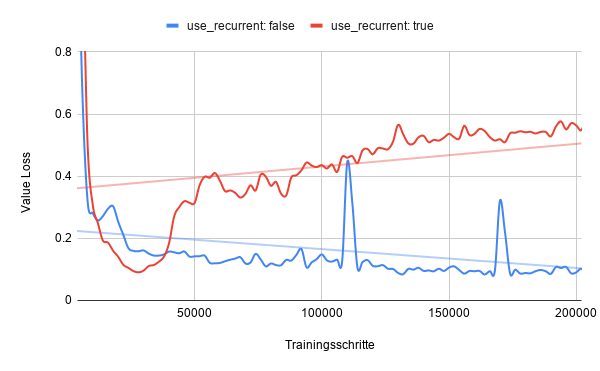
\includegraphics[scale=0.6]{images/training/base_results/result_userecurrent_loss.png}
\caption{Verlauf des Value Loss, Anpassung von \Fachbegriff{use\_recurrent}}
\label{fig:result_userecurrent_loss}
\end{figure}

\begin{figure}[H]
\centering
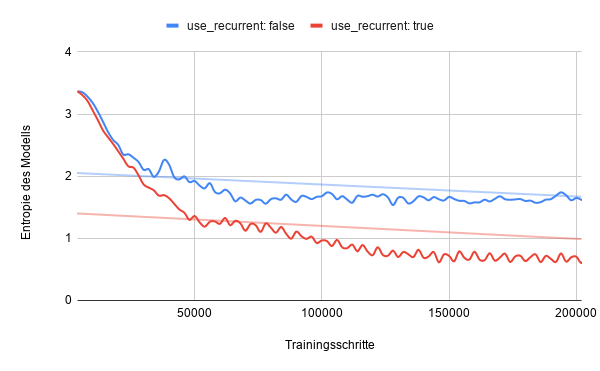
\includegraphics[scale=0.6]{images/training/base_results/result_userecurrent_entropy.png}
\caption{Entropieverlauf, Anpassung von \Fachbegriff{use\_recurrent}}
\label{fig:result_userecurrent_entropy}
\end{figure}

Insgesamt hat sich der Verlauf der Belohnungsfunktion stark verschlechtert. Die Kurve des Value Loss steigt nach einem initialen Abstieg stark an und erzielt schlussendlich ein extrem schlechtes Ergebnis. Zwar wird eine niedrigerer Wert für die Entropie erreicht, doch insgesamt ist das Ergebnis nicht akzeptabel. Daher wird von der Nutzung von rekurrenten Netzen abgesehen. Tatsächlich wurde durch das Training ein so viel schlechteres Ergebnis erzielt, dass von einer weiteren Anpassung der Parameter bezüglich rekurrenter Netze abgesehen wird.



\subsection*{Gamma}
Um den Einfluss zukünftiger Belohnungen auf die Entscheidungen des Agenten zu beeinflussen, wird der Parameter Gamma ($\gamma$) angepasst (siehe Abschnitt \ref{markov_decision_problems}). 

\begin{figure}[H]
\centering
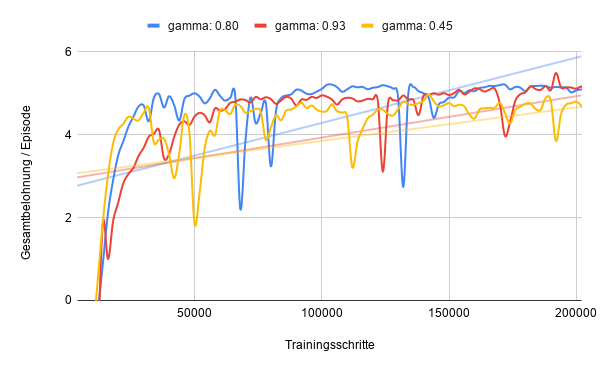
\includegraphics[scale=0.6]{images/training/base_results/result_gamma_rewards.png}
\caption{Belohnungsverlauf, Anpassung von \Fachbegriff{gamma}}
\label{fig:result_gamma_rewards}
\end{figure}

\begin{figure}[H]
\centering
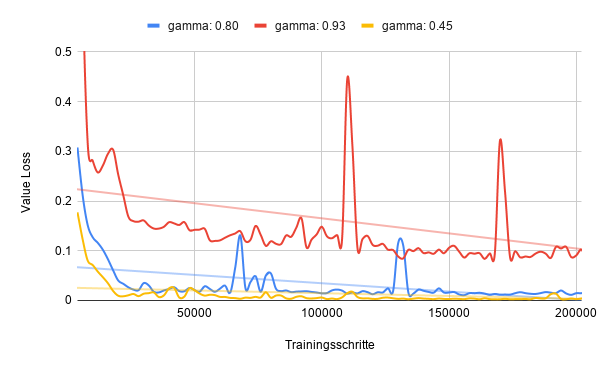
\includegraphics[scale=0.6]{images/training/base_results/result_gamma_loss.png}
\caption{Entropieverlauf, Anpassung von \Fachbegriff{gamma}}
\label{fig:result_gamma_loss}
\end{figure}

\begin{figure}[H]
\centering
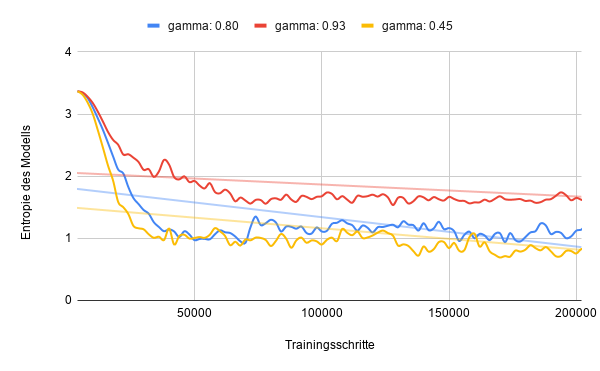
\includegraphics[scale=0.6]{images/training/base_results/result_gamma_entropy.png}
\caption{Verlauf des Value Loss, Anpassung von \Fachbegriff{gamma}}
\label{fig:result_gamma_entropy}
\end{figure}

An dem Entropieverlauf ist klar zu erkennen, dass die Wahl eines niedrigen Werts für $\gamma$ zu einem besseren Ergebnis führt. Ebenso verhält es sich mit der Entropie. Der Graph, der den niedrigsten Wert mit $\gamma = 0.45$ repräsentiert, zeigt das beste Ergebnis. Gleichzeitig erzielt der Trainingsvorgang mit diesem Wert deutlich schlechtere Werte für den Belohnungsverlauf. Das beste Ergebnis wird hier von dem Graphen erreicht, der durch den Wert $\gamma = 0.80$ entstanden ist. $\gamma$ wird daher auf diesen Wert festgelegt.



\subsection*{Größe der Batches}
Verschiedene Parameter innerhalb des empfohlenen Intervalls für den Parameter \Fachbegriff{batch\_size} wurden getestet. Die Ergebnisse sind im Folgenden zu erkennen:

\begin{figure}[H]
\centering
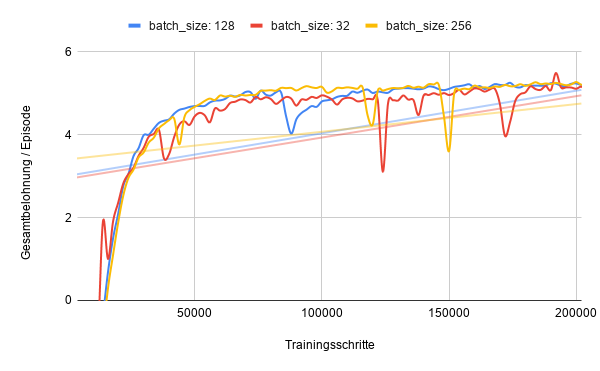
\includegraphics[scale=0.6]{images/training/base_results/result_batchsize_rewards.png}
\caption{Belohnungsverlauf, Anpassung von \Fachbegriff{batch\_size}}
\label{fig:result_batchsize_rewards}
\end{figure}

\begin{figure}[H]
\centering
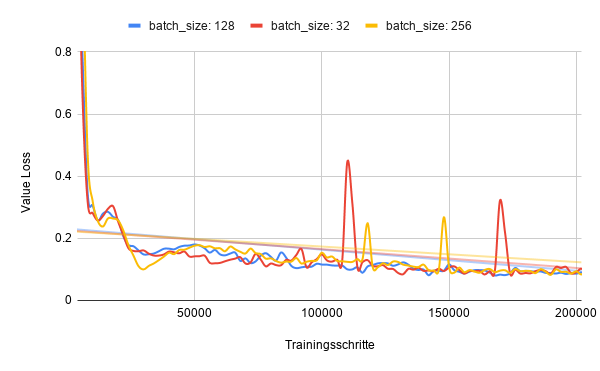
\includegraphics[scale=0.6]{images/training/base_results/result_batchsize_loss.png}
\caption{Verlauf des Value Loss, Anpassung von \Fachbegriff{batch\_size}}
\label{fig:result_batchsize_loss}
\end{figure}

\begin{figure}[H]
\centering
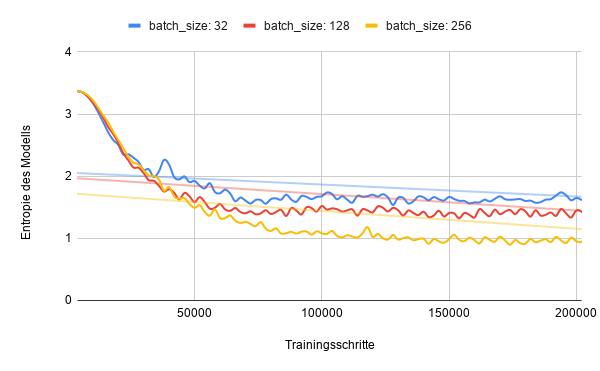
\includegraphics[scale=0.6]{images/training/base_results/result_batchsize_entropy.png}
\caption{Entropieverlauf, Anpassung von \Fachbegriff{batch\_size}}
\label{fig:result_batchsize_entropy}
\end{figure}

Es ist deutlich zu erkennen, dass sich für die höchste \Fachbegriff{batch\_size} die am wenigsten zufälligen Entscheidungen ergeben. Die Verläufe der Value Loss- und Belohnungsfunktionen sind weitestgehend identisch. Daher wird eine Batchgröße von 256 gewählt.



\subsection*{Beta}
Weiterhin wurden verschiedene Wert für den Parameter Beta ($\beta$) ausprobiert. Das Resultat ist in den folgenden Abbildungen erkennbar:

\begin{figure}[H]
\centering
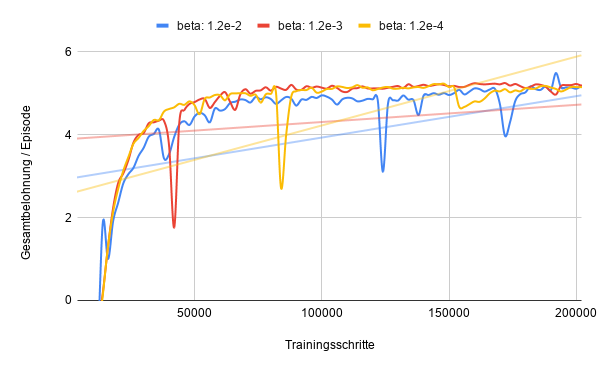
\includegraphics[scale=0.6]{images/training/base_results/result_beta_rewards.png}
\caption{Belohnungsverlauf, Anpassung von \Fachbegriff{beta}}
\label{fig:result_beta_rewards}
\end{figure}

\begin{figure}[H]
\centering
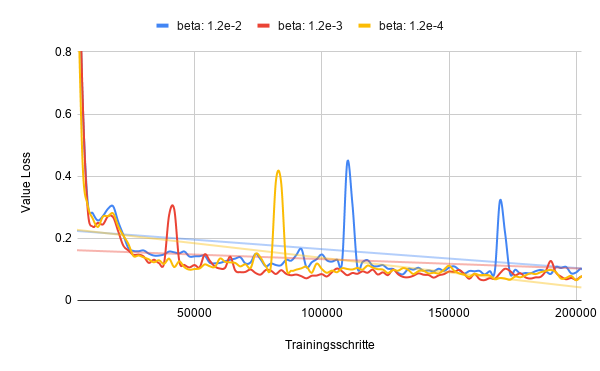
\includegraphics[scale=0.6]{images/training/base_results/result_beta_loss.png}
\caption{Verlauf des Value Loss, Anpassung von \Fachbegriff{beta}}
\label{fig:result_beta_loss}
\end{figure}

\begin{figure}[H]
\centering
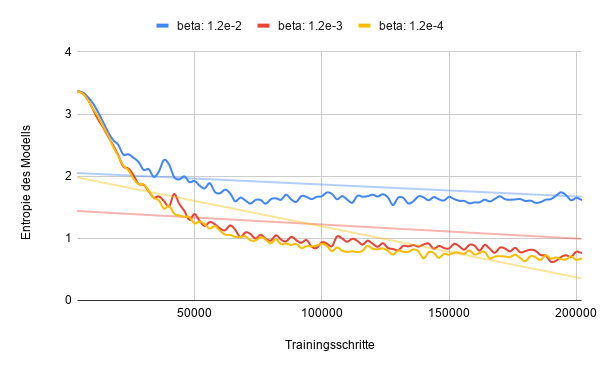
\includegraphics[scale=0.6]{images/training/base_results/result_beta_entropy.png}
\caption{Entropieverlauf, Anpassung von \Fachbegriff{beta}}
\label{fig:result_beta_entropy}
\end{figure}


Insgesamt konnten mit niedrigeren Werten für $\beta$ schneller ein besseres Ergebnis erzielt werden. Das gilt für die Belohnungsfunktion, den Value Loss und die Entropie des Modells. Da für den Wert $\beta = 1.2e-3$ jedoch höhere Belohnungen als für den Wert $\beta = 1.2e-4$ erreicht wurden, wird Beta auf den Wert $\beta = 1.2e-3$ festgelegt.



\subsection*{Lambda}
Der Parameter Lambda ($\lambda$) wurde ebenfalls angepasst, wie in den folgenden Grafiken zu erkennen:

\begin{figure}[H]
\centering
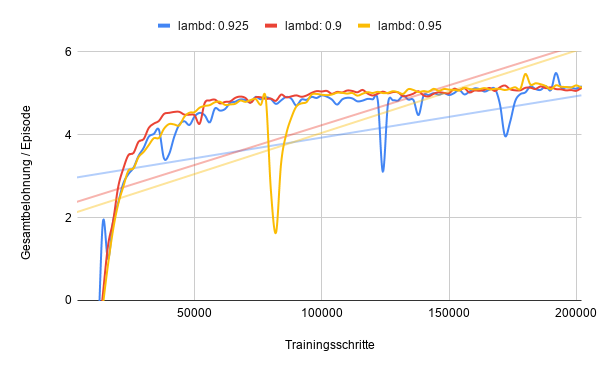
\includegraphics[scale=0.6]{images/training/base_results/result_lambd_rewards.png}
\caption{Belohnungsverlauf, Anpassung von \Fachbegriff{lambd}}
\label{fig:result_lambd_rewards}
\end{figure}

\begin{figure}[H]
\centering
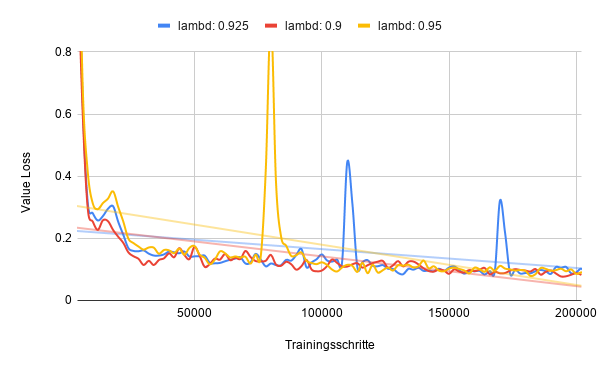
\includegraphics[scale=0.6]{images/training/base_results/result_lambd_loss.png}
\caption{Verlauf des Value Loss, Anpassung von \Fachbegriff{lambd}}
\label{fig:result_lambd_loss}
\end{figure}

\begin{figure}[H]
\centering
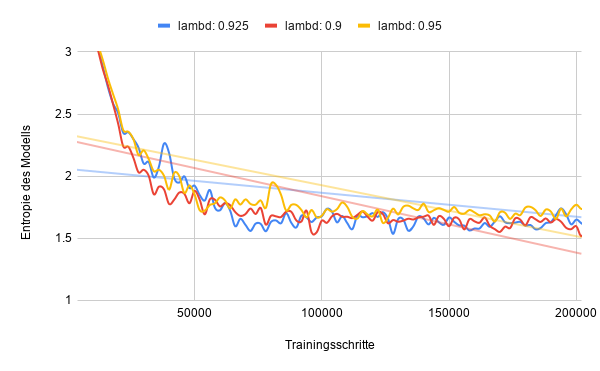
\includegraphics[scale=0.6]{images/training/base_results/result_lambd_entropy.png}
\caption{Entropieverlauf, Anpassung von \Fachbegriff{lambd}}
\label{fig:result_lambd_entropy}
\end{figure}

Die Belohnungsfunktion stabilisiert sich leicht durch die Verwendung eine niedrigeren Wertes für $\lambda$. Auch für die Value Loss- und Entropiefunktion ergibt sich ein leicht verbessertes Ergebnis. Der niedrigste Wert $\lambda = 0.9$ führt also insgesamt zum besten Ergebnis.



\subsection*{Anzahl der Epochen}
Ein weiterer Trainingsdurchlauf wird mit einer reduzierten Anzahl \Fachbegriff{num\_epoch} von vier auf drei Epochen durchgeführt. Dadurch wird derselbe Buffer weniger oft für den Gradientenabstieg verwendet. Geringere Werte sollten in einem stabileren, aber langsameren Training resultieren. ML-Agents empfiehlt einen Minimalwert von $\Fachbegriff{num\_epoch} = 3$.

\begin{figure}[H]
\centering
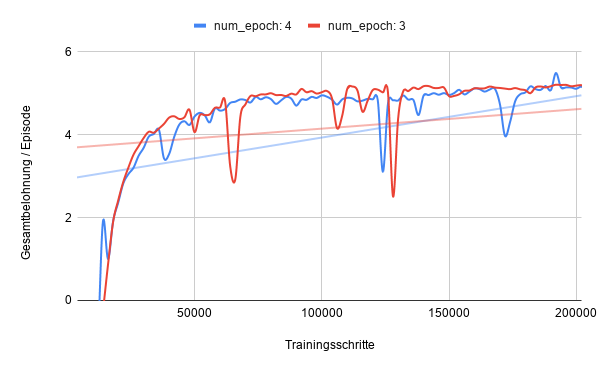
\includegraphics[scale=0.6]{images/training/base_results/result_numepochs_rewards.png}
\caption{Belohnungsverlauf, Anpassung von \Fachbegriff{num\_epochs}}
\label{fig:result_numepochs_rewards}
\end{figure}

\begin{figure}[H]
\centering
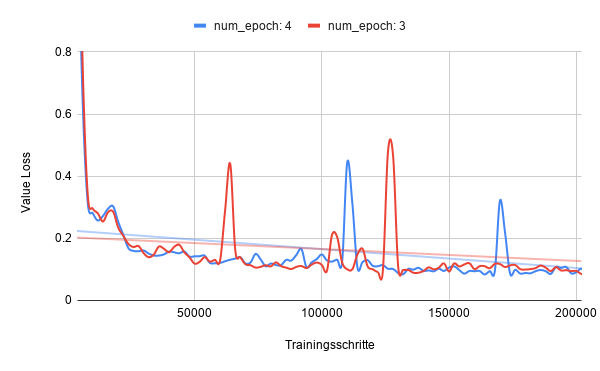
\includegraphics[scale=0.6]{images/training/base_results/result_numepochs_loss.png}
\caption{Verlauf des Value Loss, Anpassung von \Fachbegriff{num\_epochs}}
\label{fig:result_numepochs_loss}
\end{figure}

\begin{figure}[H]
\centering
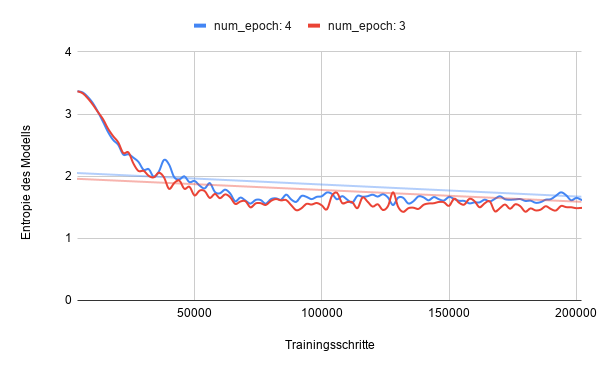
\includegraphics[scale=0.6]{images/training/base_results/result_numepochs_entropy.png}
\caption{Entropieverlauf, Anpassung von \Fachbegriff{num\_epochs}}
\label{fig:result_numepochs_entropy}
\end{figure}

Da die Belohnungsfunktion schneller ansteigt und insgesamt einen hohen Level erreicht und wegen der leicht verbesserten Entropie, wird der Parameter \Fachbegriff{num\_epoch} auf $3$ festgelegt. 



\subsection*{Epsilon}
Der Hyperparameter \Fachbegriff{epsilon} wird angepasst, um zu bestimmen, wie schnell sich eine Policy im Verlauf des Trainings verändern darf. Die Ergebnisse sind in den folgenden Abbildungen zu erkennen:

\begin{figure}[H]
\centering
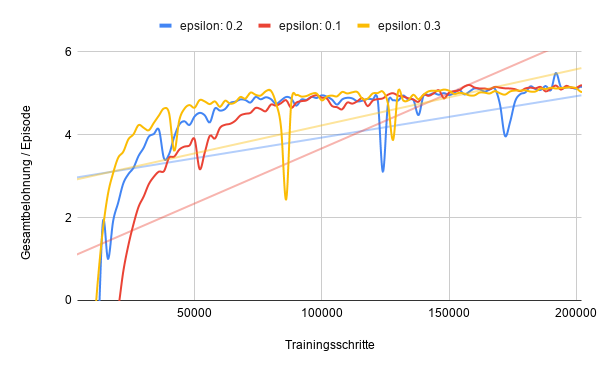
\includegraphics[scale=0.6]{images/training/base_results/result_epsilon_rewards.png}
\caption{Belohnungsverlauf, Anpassung von \Fachbegriff{epsilon}}
\label{fig:result_epsilon_rewards}
\end{figure}

\begin{figure}[H]
\centering
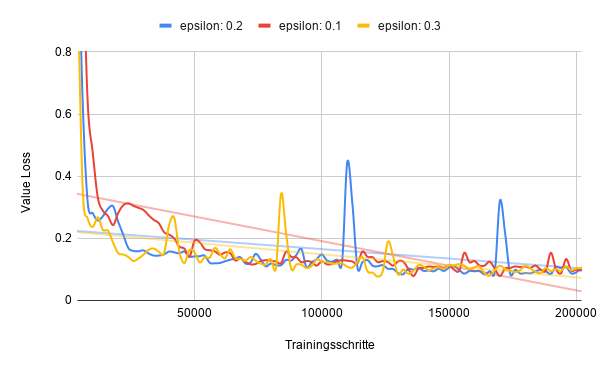
\includegraphics[scale=0.6]{images/training/base_results/result_epsilon_loss.png}
\caption{Verlauf des Value Loss, Anpassung von \Fachbegriff{epsilon}}
\label{fig:result_epsilon_loss}
\end{figure}

\begin{figure}[H]
\centering
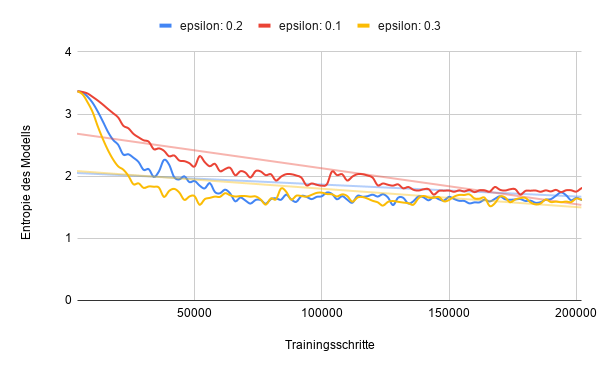
\includegraphics[scale=0.6]{images/training/base_results/result_epsilon_entropy.png}
\caption{Entropieverlauf, Anpassung von \Fachbegriff{epsilon}}
\label{fig:result_epsilon_entropy}
\end{figure}

Wenn der Wert $0.3$ für den Parameter \Fachbegriff{epsilon} gewählt wird, erfolgen daraus insgesamt leicht verbesserte Ergebnisse für alle drei Metriken. Weiterhin wird die Geschwindigkeit des Lernvorgangs erhöht. Dieser Wert wird daher für das finale Training verwendet.




\subsection*{Größe des Buffers}
Weiterhin wird die Größe des Buffers angepasst, um die Auswirkungen dieser Änderungen im Training zu betrachten.

\begin{figure}[H]
\centering
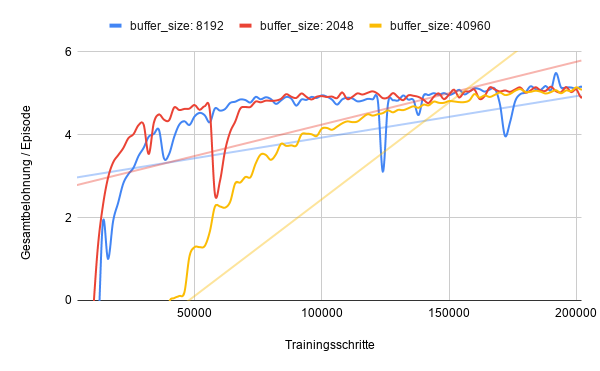
\includegraphics[scale=0.6]{images/training/base_results/result_buffer_rewards.png}
\caption{Belohnungsverlauf, Anpassung von \Fachbegriff{buffer\_size}}
\label{fig:result_buffer_rewards}
\end{figure}

\begin{figure}[H]
\centering
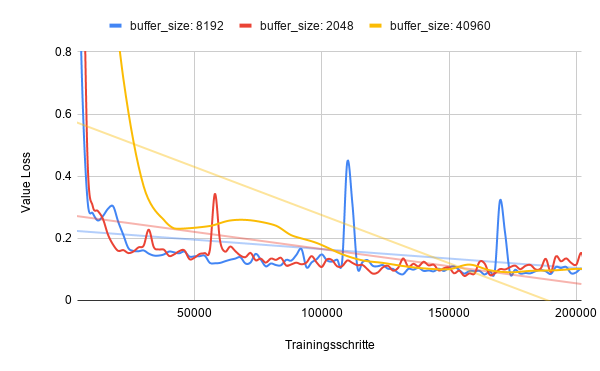
\includegraphics[scale=0.6]{images/training/base_results/result_buffer_loss.png}
\caption{Verlauf des Value Loss, Anpassung von \Fachbegriff{buffer\_size}}
\label{fig:result_buffer_loss}
\end{figure}

\begin{figure}[H]
\centering
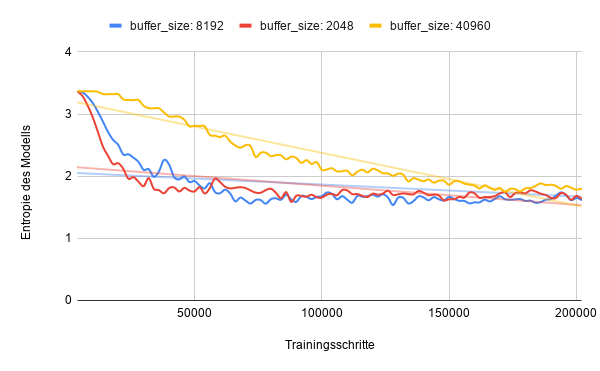
\includegraphics[scale=0.6]{images/training/base_results/result_buffer_entropy.png}
\caption{Entropieverlauf, Anpassung von \Fachbegriff{buffer\_size}}
\label{fig:result_buffer_entropy}
\end{figure}

Die höchste Buffergröße führt zu einem deutlich verlangsamten Trainingsvorgang mit insgesamt schlechteren Ergebnissen für Belohnungen, Value Loss und die Entropie.
Für niedrige Werte erfolgt ein leicht schnellerer Lernvorgang mit ähnlichen Endergebnissen für die Belohnungswerte. Da sich die Entropie und der Value Loss jedoch nicht verändern, wird weiterhin der Wert $8192$ für die Buffergröße gewählt.
